\section{Go as a state of the art non-preemptively scheduled language}
Go is a state of the art web-centered language which exclusively handles concurrency through user-space context-switching. It was created at Google in 2010 by some of the computer science pioneers that originally came up with Unix and C at Bell Labs, so it is no surprise that Go has been described as a "\textit{C-like language}" or as "\textit{C for the 21st Century}" \cite{GoPL2015}. 

Furthermore, it was created with "built-in concurrency" to tackle modern large distributed infrastructure problems and it is currently widely used at all network traffic levels as a server-side service provider \cite{Pike2012}\cite{Ajmani2016}\cite{2022DataRacesGolang}. Therefore, it is a great candidate as a point of reference of how modern server-side network concurrency can be handled exclusively in user-space \cite{GoArticleACM}, particularly when compared to a preemptively scheduled application in its 'close-relative' C.

\subsection{Goroutines}
\begin{figure}[!t]
	\centering
	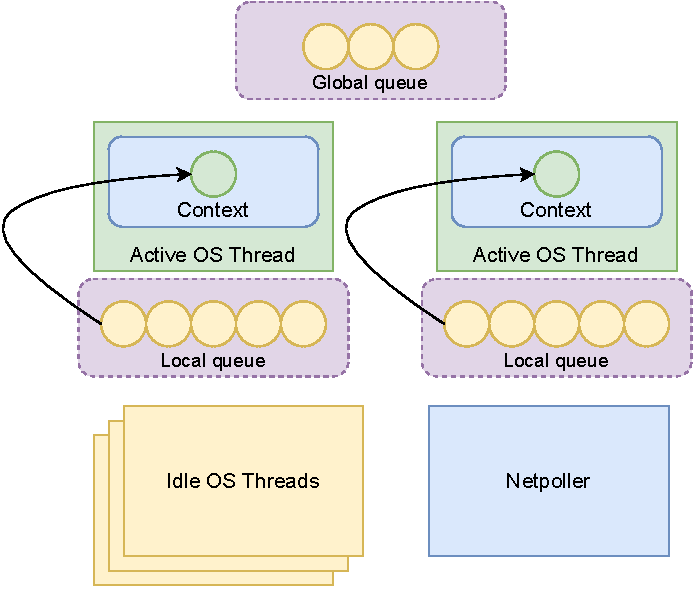
\includegraphics[width=2.5in]{img/go_runtime.pdf}
	%where an .eps filename suffix will be assumed under latex, 
	%and a .pdf suffix will be assumed for pdflatex; or what has been declared
	%via \DeclareGraphicsExtensions.
	\caption{High level depiction of the runtime environment in Go. \textit{Goroutines} are depicted as circles, OS threads as rectangles. Active goroutines running on a \textit{context} are green, idle goroutines waiting in a queue are yellow. The same color semantics apply to active and idle OS threads.}
	\label{fig_go_runtime}
\end{figure}
The idiomatic way of dealing with client connections in a Go server, is by spawning a new \textit{goroutine} that handles each client concurrently \cite{Morsing2013_2}\cite{GoNet}. Goroutines are very lightweight concurrent subroutines supervised by the Go \textit{runtime} exclusively in user-space. Their memory footprint is very small \cite{2013ContextSwitching}, the assigned stack memory by default is only a few kilobytes at their creation \cite{Cox-Buday2017}. 

Goroutines are non-preemptive, i.e. they are not interrupted by the operating system's (OS) scheduler to run other goroutines. They have defined \textit{points of entry} where they can be suspended or activated by Go's runtime scheduler, which is entirely running in user-space. Since a context-switch between goroutines happens in user-space and the runtime decides which data should be persistent between context-switches, it can be orders of magnitude faster than context-switching between OS threads \cite{Cox-Buday2017} or between OS processes \cite{Kerrisk2010}. A context-switch between OS threads or processes is a costly operation in terms of both the kernel-side data structures needed to manage all threads and processes and the operations performed in kernel-space to make the transition happen.

\subsection{Runtime scheduler}
Each Go executable is compiled with its own statically linked runtime environment in charge of scheduling the goroutines, garbage collection and other tasks. The system model that describes the runtime scheduler consists of three main elements: goroutines, contexts and the OS threads where the goroutines are run. Goroutines are placed by the runtime in either the local queue of a context or in the global queue pending to be run by a context in one of the OS threads, as illustrated in figure \ref{fig_go_runtime}. The contexts are in charge of managing the scheduling of the queues and the data required by the different goroutines.

Parallelism in the system is achieved by having multiple contexts (in fig. \ref{fig_go_runtime} only two contexts are simultaneously running, depicted as blue rectangles), each using a different core of the processor through different OS threads. The runtime manages a set of working threads (illustrated as green rectangles) coupled with contexts and another set of idle threads (yellow rectangles).  If a goroutine performs a syscall that would block, e.g. listening for clients on a TCP socket, the underlying OS thread in which the context is executing the goroutine would also have to block. In this scenario, the blocking thread is decoupled from the context, so that the context can re-activate one of the idle threads and keep working with other non-blocking goroutines.

As long as the goroutines running in the contexts do not call a blocking system call, the different goroutines in the queues can be freely interchanged by the scheduler at the given \textit{points of entry} within the same set of OS threads. This, as previously stated, avoids a costly context-switch in kernel-space. 

Nonetheless, blocking syscalls for networking are handled in a special way by the runtime. If the server were to have thousands of simultaneously connected clients and most of the clients were to call blocking system calls at the same time, it would then have to create a unique blocked OS thread for each client. This state would be very costly because every blocked client goroutine would translate to one blocked OS thread, consequently defeating Go's goal of keeping context-switches primarily in user-space.

Therefore, Go handles network connections in a way that avoids using too many system resources. When a goroutine tries to read from a client socket which would block, a special perpetually running thread called the "\textit{netpoller}" is notified of this fact \cite{Morsing2013_2} (the netpoller thread is depicted as a blue rectangle in fig. \ref{fig_go_runtime}). The goroutine which could not perform its network operation is placed back on a queue (making its OS thread once again free to run another goroutine). The netpoller continually polls all network sockets and notifies a context when an operation on the socket would not block, so that the goroutine can be scheduled back in the future. Thereupon, the runtime environment avoids overloading the kernel with unnecessarily too many blocked threads for the client connections.

After getting to know the complex concurrency abstractions and the runtime system that were developed to allegedly perform well in highly-concurrent network systems, one might ask: how does this state of the art concurrency paradigm compare performance-wise with a traditional multi-procedural framework?